\documentclass[1p]{elsarticle_modified}
%\bibliographystyle{elsarticle-num}

%\usepackage[colorlinks]{hyperref}
%\usepackage{abbrmath_seonhwa} %\Abb, \Ascr, \Acal ,\Abf, \Afrak
\usepackage{amsfonts}
\usepackage{amssymb}
\usepackage{amsmath}
\usepackage{amsthm}
\usepackage{scalefnt}
\usepackage{amsbsy}
\usepackage{kotex}
\usepackage{caption}
\usepackage{subfig}
\usepackage{color}
\usepackage{graphicx}
\usepackage{xcolor} %% white, black, red, green, blue, cyan, magenta, yellow
\usepackage{float}
\usepackage{setspace}
\usepackage{hyperref}

\usepackage{tikz}
\usetikzlibrary{arrows}

\usepackage{multirow}
\usepackage{array} % fixed length table
\usepackage{hhline}

%%%%%%%%%%%%%%%%%%%%%
\makeatletter
\renewcommand*\env@matrix[1][\arraystretch]{%
	\edef\arraystretch{#1}%
	\hskip -\arraycolsep
	\let\@ifnextchar\new@ifnextchar
	\array{*\c@MaxMatrixCols c}}
\makeatother %https://tex.stackexchange.com/questions/14071/how-can-i-increase-the-line-spacing-in-a-matrix
%%%%%%%%%%%%%%%

\usepackage[normalem]{ulem}

\newcommand{\msout}[1]{\ifmmode\text{\sout{\ensuremath{#1}}}\else\sout{#1}\fi}
%SOURCE: \msout is \stkout macro in https://tex.stackexchange.com/questions/20609/strikeout-in-math-mode

\newcommand{\cancel}[1]{
	\ifmmode
	{\color{red}\msout{#1}}
	\else
	{\color{red}\sout{#1}}
	\fi
}

\newcommand{\add}[1]{
	{\color{blue}\uwave{#1}}
}

\newcommand{\replace}[2]{
	\ifmmode
	{\color{red}\msout{#1}}{\color{blue}\uwave{#2}}
	\else
	{\color{red}\sout{#1}}{\color{blue}\uwave{#2}}
	\fi
}

\newcommand{\Sol}{\mathcal{S}} %segment
\newcommand{\D}{D} %diagram
\newcommand{\A}{\mathcal{A}} %arc


%%%%%%%%%%%%%%%%%%%%%%%%%%%%%5 test

\def\sl{\operatorname{\textup{SL}}(2,\Cbb)}
\def\psl{\operatorname{\textup{PSL}}(2,\Cbb)}
\def\quan{\mkern 1mu \triangleright \mkern 1mu}

\theoremstyle{definition}
\newtheorem{thm}{Theorem}[section]
\newtheorem{prop}[thm]{Proposition}
\newtheorem{lem}[thm]{Lemma}
\newtheorem{ques}[thm]{Question}
\newtheorem{cor}[thm]{Corollary}
\newtheorem{defn}[thm]{Definition}
\newtheorem{exam}[thm]{Example}
\newtheorem{rmk}[thm]{Remark}
\newtheorem{alg}[thm]{Algorithm}

\newcommand{\I}{\sqrt{-1}}
\begin{document}

%\begin{frontmatter}
%
%\title{Boundary parabolic representations of knots up to 8 crossings}
%
%%% Group authors per affiliation:
%\author{Yunhi Cho} 
%\address{Department of Mathematics, University of Seoul, Seoul, Korea}
%\ead{yhcho@uos.ac.kr}
%
%
%\author{Seonhwa Kim} %\fnref{s_kim}}
%\address{Center for Geometry and Physics, Institute for Basic Science, Pohang, 37673, Korea}
%\ead{ryeona17@ibs.re.kr}
%
%\author{Hyuk Kim}
%\address{Department of Mathematical Sciences, Seoul National University, Seoul 08826, Korea}
%\ead{hyukkim@snu.ac.kr}
%
%\author{Seokbeom Yoon}
%\address{Department of Mathematical Sciences, Seoul National University, Seoul, 08826,  Korea}
%\ead{sbyoon15@snu.ac.kr}
%
%\begin{abstract}
%We find all boundary parabolic representation of knots up to 8 crossings.
%
%\end{abstract}
%\begin{keyword}
%    \MSC[2010] 57M25 
%\end{keyword}
%
%\end{frontmatter}

%\linenumbers
%\tableofcontents
%
\newcommand\colored[1]{\textcolor{white}{\rule[-0.35ex]{0.8em}{1.4ex}}\kern-0.8em\color{red} #1}%
%\newcommand\colored[1]{\textcolor{white}{ #1}\kern-2.17ex	\textcolor{white}{ #1}\kern-1.81ex	\textcolor{white}{ #1}\kern-2.15ex\color{red}#1	}

{\Large $\underline{12n_{0394}~(K12n_{0394})}$}

\setlength{\tabcolsep}{10pt}
\renewcommand{\arraystretch}{1.6}
\vspace{1cm}\begin{tabular}{m{100pt}>{\centering\arraybackslash}m{274pt}}
\multirow{5}{120pt}{
	\centering
	\includegraphics[width=112pt]{../../../GIT/diagram.site/Diagrams/png/2483_12n_0394.png}\\
\ \ \ A knot diagram\footnotemark}&
\allowdisplaybreaks
\textbf{Linearized knot diagam} \\
\cline{2-2}
 &
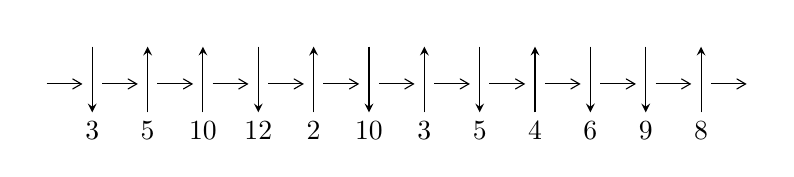
\begin{tikzpicture}[x=20pt, y=17pt]
	% nodes
	\node (C0) at (0, 0) {};
	\node (C1) at (1, 0) {};
	\node (C1U) at (1, +1) {};
	\node (C1D) at (1, -1) {3};

	\node (C2) at (2, 0) {};
	\node (C2U) at (2, +1) {};
	\node (C2D) at (2, -1) {5};

	\node (C3) at (3, 0) {};
	\node (C3U) at (3, +1) {};
	\node (C3D) at (3, -1) {10};

	\node (C4) at (4, 0) {};
	\node (C4U) at (4, +1) {};
	\node (C4D) at (4, -1) {12};

	\node (C5) at (5, 0) {};
	\node (C5U) at (5, +1) {};
	\node (C5D) at (5, -1) {2};

	\node (C6) at (6, 0) {};
	\node (C6U) at (6, +1) {};
	\node (C6D) at (6, -1) {10};

	\node (C7) at (7, 0) {};
	\node (C7U) at (7, +1) {};
	\node (C7D) at (7, -1) {3};

	\node (C8) at (8, 0) {};
	\node (C8U) at (8, +1) {};
	\node (C8D) at (8, -1) {5};

	\node (C9) at (9, 0) {};
	\node (C9U) at (9, +1) {};
	\node (C9D) at (9, -1) {4};

	\node (C10) at (10, 0) {};
	\node (C10U) at (10, +1) {};
	\node (C10D) at (10, -1) {6};

	\node (C11) at (11, 0) {};
	\node (C11U) at (11, +1) {};
	\node (C11D) at (11, -1) {9};

	\node (C12) at (12, 0) {};
	\node (C12U) at (12, +1) {};
	\node (C12D) at (12, -1) {8};
	\node (C13) at (13, 0) {};

	% arrows
	\draw[->,>={angle 60}]
	(C0) edge (C1) (C1) edge (C2) (C2) edge (C3) (C3) edge (C4) (C4) edge (C5) (C5) edge (C6) (C6) edge (C7) (C7) edge (C8) (C8) edge (C9) (C9) edge (C10) (C10) edge (C11) (C11) edge (C12) (C12) edge (C13) ;	\draw[->,>=stealth]
	(C1U) edge (C1D) (C2D) edge (C2U) (C3D) edge (C3U) (C4U) edge (C4D) (C5D) edge (C5U) (C6U) edge (C6D) (C7D) edge (C7U) (C8U) edge (C8D) (C9D) edge (C9U) (C10U) edge (C10D) (C11U) edge (C11D) (C12D) edge (C12U) ;
	\end{tikzpicture} \\
\hhline{~~} \\& 
\textbf{Solving Sequence} \\ \cline{2-2} 
 &
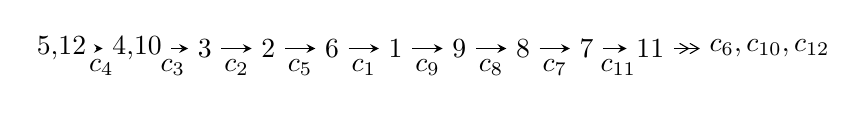
\begin{tikzpicture}[x=23pt, y=7pt]
	% node
	\node (A0) at (-1/8, 0) {5,12};
	\node (A1) at (17/16, 0) {4,10};
	\node (A2) at (17/8, 0) {3};
	\node (A3) at (25/8, 0) {2};
	\node (A4) at (33/8, 0) {6};
	\node (A5) at (41/8, 0) {1};
	\node (A6) at (49/8, 0) {9};
	\node (A7) at (57/8, 0) {8};
	\node (A8) at (65/8, 0) {7};
	\node (A9) at (73/8, 0) {11};
	\node (C1) at (1/2, -1) {$c_{4}$};
	\node (C2) at (13/8, -1) {$c_{3}$};
	\node (C3) at (21/8, -1) {$c_{2}$};
	\node (C4) at (29/8, -1) {$c_{5}$};
	\node (C5) at (37/8, -1) {$c_{1}$};
	\node (C6) at (45/8, -1) {$c_{9}$};
	\node (C7) at (53/8, -1) {$c_{8}$};
	\node (C8) at (61/8, -1) {$c_{7}$};
	\node (C9) at (69/8, -1) {$c_{11}$};
	\node (A10) at (11, 0) {$c_{6},c_{10},c_{12}$};

	% edge
	\draw[->,>=stealth]	
	(A0) edge (A1) (A1) edge (A2) (A2) edge (A3) (A3) edge (A4) (A4) edge (A5) (A5) edge (A6) (A6) edge (A7) (A7) edge (A8) (A8) edge (A9) ;
	\draw[->>,>={angle 60}]	
	(A9) edge (A10);
\end{tikzpicture} \\ 

\end{tabular} \\

\footnotetext{
The image of knot diagram is generated by the software ``\textbf{Draw programme}" developed by Andrew Bartholomew(\url{http://www.layer8.co.uk/maths/draw/index.htm\#Running-draw}), where we modified some parts for our purpose(\url{https://github.com/CATsTAILs/LinksPainter}).
}\phantom \\ \newline 
\centering \textbf{Ideals for irreducible components\footnotemark of $X_{\text{par}}$} 
 
\begin{align*}
I^u_{1}&=\langle 
5 u^{16}+50 u^{15}+\cdots+23 b-101,\;-166 u^{16}-487 u^{15}+\cdots+69 a+216,\;u^{17}+4 u^{16}+\cdots-6 u-3\rangle \\
I^u_{2}&=\langle 
u^2+b- u-2,\;a-2 u+2,\;u^3-2 u^2+u+1\rangle \\
I^u_{3}&=\langle 
b+1,\;-2 u^4 a+2 u^4+2 u^2 a- u^3+a^2-2 a u-3 a+2 u+3,\;u^5- u^4+u^2+u-1\rangle \\
I^u_{4}&=\langle 
b+1,\;-2 u^4 a+8 u^4+2 u^2 a+3 u^3+a^2+2 a u-2 u^2-3 a-8 u+11,\;u^5+u^4- u^2+u+1\rangle \\
I^u_{5}&=\langle 
b- u-1,\;a- u,\;u^2- u+1\rangle \\
\\
\end{align*}
\raggedright * 5 irreducible components of $\dim_{\mathbb{C}}=0$, with total 42 representations.\\
\footnotetext{All coefficients of polynomials are rational numbers. But the coefficients are sometimes approximated in decimal forms when there is not enough margin.}
\newpage
\renewcommand{\arraystretch}{1}
\centering \section*{I. $I^u_{1}= \langle 5 u^{16}+50 u^{15}+\cdots+23 b-101,\;-166 u^{16}-487 u^{15}+\cdots+69 a+216,\;u^{17}+4 u^{16}+\cdots-6 u-3 \rangle$}
\flushleft \textbf{(i) Arc colorings}\\
\begin{tabular}{m{7pt} m{180pt} m{7pt} m{180pt} }
\flushright $a_{5}=$&$\begin{pmatrix}1\\0\end{pmatrix}$ \\
\flushright $a_{12}=$&$\begin{pmatrix}0\\u\end{pmatrix}$ \\
\flushright $a_{4}=$&$\begin{pmatrix}1\\- u^2\end{pmatrix}$ \\
\flushright $a_{10}=$&$\begin{pmatrix}2.40580 u^{16}+7.05797 u^{15}+\cdots-7.44928 u-3.13043\\-0.217391 u^{16}-2.17391 u^{15}+\cdots+2.34783 u+4.39130\end{pmatrix}$ \\
\flushright $a_{3}=$&$\begin{pmatrix}1.53623 u^{16}+6.36232 u^{15}+\cdots-7.05797 u-8.56522\\1.39130 u^{16}+4.91304 u^{15}+\cdots-5.82609 u-3.30435\end{pmatrix}$ \\
\flushright $a_{2}=$&$\begin{pmatrix}0.144928 u^{16}+1.44928 u^{15}+\cdots-1.23188 u-5.26087\\1.39130 u^{16}+4.91304 u^{15}+\cdots-5.82609 u-3.30435\end{pmatrix}$ \\
\flushright $a_{6}=$&$\begin{pmatrix}1.89855 u^{16}+6.98551 u^{15}+\cdots-9.63768 u-6.21739\\0.304348 u^{16}+0.0434783 u^{15}+\cdots-0.0869565 u+2.65217\end{pmatrix}$ \\
\flushright $a_{1}=$&$\begin{pmatrix}-0.971014 u^{16}-2.71014 u^{15}+\cdots+2.75362 u+4.34783\\0.782609 u^{16}+1.82609 u^{15}+\cdots-1.65217 u-0.608696\end{pmatrix}$ \\
\flushright $a_{9}=$&$\begin{pmatrix}1.01449 u^{16}+2.14493 u^{15}+\cdots-1.62319 u+0.173913\\-1.13043 u^{16}-3.30435 u^{15}+\cdots+2.60870 u+2.43478\end{pmatrix}$ \\
\flushright $a_{8}=$&$\begin{pmatrix}-0.115942 u^{16}-1.15942 u^{15}+\cdots+0.985507 u+2.60870\\-1.13043 u^{16}-3.30435 u^{15}+\cdots+2.60870 u+2.43478\end{pmatrix}$ \\
\flushright $a_{7}=$&$\begin{pmatrix}-1.60870 u^{16}-5.08696 u^{15}+\cdots+9.17391 u+5.69565\\1.82609 u^{16}+5.26087 u^{15}+\cdots-5.52174 u-5.08696\end{pmatrix}$ \\
\flushright $a_{11}=$&$\begin{pmatrix}-2.40580 u^{16}-7.05797 u^{15}+\cdots+9.44928 u+7.13043\\0.652174 u^{16}+2.52174 u^{15}+\cdots-3.04348 u-2.17391\end{pmatrix}$\\&\end{tabular}
\flushleft \textbf{(ii) Obstruction class $= -1$}\\~\\
\flushleft \textbf{(iii) Cusp Shapes $= \frac{117}{23} u^{16}+\frac{365}{23} u^{15}+\cdots-\frac{592}{23} u-\frac{459}{23}$}\\~\\
\newpage\renewcommand{\arraystretch}{1}
\flushleft \textbf{(iv) u-Polynomials at the component}\newline \\
\begin{tabular}{m{50pt}|m{274pt}}
Crossings & \hspace{64pt}u-Polynomials at each crossing \\
\hline $$\begin{aligned}c_{1}\end{aligned}$$&$\begin{aligned}
&u^{17}+16 u^{16}+\cdots+10 u-1
\end{aligned}$\\
\hline $$\begin{aligned}c_{2},c_{3},c_{5}\\c_{9}\end{aligned}$$&$\begin{aligned}
&u^{17}+8 u^{15}+\cdots+4 u+1
\end{aligned}$\\
\hline $$\begin{aligned}c_{4}\end{aligned}$$&$\begin{aligned}
&u^{17}+4 u^{16}+\cdots-6 u-3
\end{aligned}$\\
\hline $$\begin{aligned}c_{6},c_{8},c_{10}\end{aligned}$$&$\begin{aligned}
&u^{17}+u^{16}+\cdots-5 u+3
\end{aligned}$\\
\hline $$\begin{aligned}c_{7}\end{aligned}$$&$\begin{aligned}
&u^{17}- u^{16}+\cdots-32 u+32
\end{aligned}$\\
\hline $$\begin{aligned}c_{11}\end{aligned}$$&$\begin{aligned}
&u^{17}-4 u^{16}+\cdots-20 u+4
\end{aligned}$\\
\hline $$\begin{aligned}c_{12}\end{aligned}$$&$\begin{aligned}
&u^{17}- u^{16}+\cdots-8 u^2+1
\end{aligned}$\\
\hline
\end{tabular}\\~\\
\newpage\renewcommand{\arraystretch}{1}
\flushleft \textbf{(v) Riley Polynomials at the component}\newline \\
\begin{tabular}{m{50pt}|m{274pt}}
Crossings & \hspace{64pt}Riley Polynomials at each crossing \\
\hline $$\begin{aligned}c_{1}\end{aligned}$$&$\begin{aligned}
&y^{17}+12 y^{16}+\cdots+582 y-1
\end{aligned}$\\
\hline $$\begin{aligned}c_{2},c_{3},c_{5}\\c_{9}\end{aligned}$$&$\begin{aligned}
&y^{17}+16 y^{16}+\cdots+10 y-1
\end{aligned}$\\
\hline $$\begin{aligned}c_{4}\end{aligned}$$&$\begin{aligned}
&y^{17}-4 y^{16}+\cdots+30 y-9
\end{aligned}$\\
\hline $$\begin{aligned}c_{6},c_{8},c_{10}\end{aligned}$$&$\begin{aligned}
&y^{17}+9 y^{16}+\cdots-77 y-9
\end{aligned}$\\
\hline $$\begin{aligned}c_{7}\end{aligned}$$&$\begin{aligned}
&y^{17}+49 y^{16}+\cdots+512 y-1024
\end{aligned}$\\
\hline $$\begin{aligned}c_{11}\end{aligned}$$&$\begin{aligned}
&y^{17}+28 y^{15}+\cdots+192 y-16
\end{aligned}$\\
\hline $$\begin{aligned}c_{12}\end{aligned}$$&$\begin{aligned}
&y^{17}-13 y^{16}+\cdots+16 y-1
\end{aligned}$\\
\hline
\end{tabular}\\~\\
\newpage\flushleft \textbf{(vi) Complex Volumes and Cusp Shapes}
$$\begin{array}{c|c|c}  
\text{Solutions to }I^u_{1}& \I (\text{vol} + \sqrt{-1}CS) & \text{Cusp shape}\\
 \hline 
\begin{aligned}
u &= -0.646906 + 0.777899 I \\
a &= \phantom{-}0.092542 + 0.678674 I \\
b &= -0.777189 + 0.739752 I\end{aligned}
 & \phantom{-}0.36478 + 1.63051 I & \phantom{-}1.33246 - 2.97241 I \\ \hline\begin{aligned}
u &= -0.646906 - 0.777899 I \\
a &= \phantom{-}0.092542 - 0.678674 I \\
b &= -0.777189 - 0.739752 I\end{aligned}
 & \phantom{-}0.36478 - 1.63051 I & \phantom{-}1.33246 + 2.97241 I \\ \hline\begin{aligned}
u &= \phantom{-}0.784984 + 0.477130 I \\
a &= -1.94672 - 0.49177 I \\
b &= \phantom{-}0.452575 + 0.318517 I\end{aligned}
 & -11.20970 - 1.90455 I & -7.06546 + 3.61390 I \\ \hline\begin{aligned}
u &= \phantom{-}0.784984 - 0.477130 I \\
a &= -1.94672 + 0.49177 I \\
b &= \phantom{-}0.452575 - 0.318517 I\end{aligned}
 & -11.20970 + 1.90455 I & -7.06546 - 3.61390 I \\ \hline\begin{aligned}
u &= \phantom{-}0.026724 + 0.844372 I \\
a &= \phantom{-}0.015923 + 0.426626 I \\
b &= \phantom{-}0.443696 + 0.862498 I\end{aligned}
 & \phantom{-}0.663995 + 1.197200 I & \phantom{-}5.46705 - 5.78482 I \\ \hline\begin{aligned}
u &= \phantom{-}0.026724 - 0.844372 I \\
a &= \phantom{-}0.015923 - 0.426626 I \\
b &= \phantom{-}0.443696 - 0.862498 I\end{aligned}
 & \phantom{-}0.663995 - 1.197200 I & \phantom{-}5.46705 + 5.78482 I \\ \hline\begin{aligned}
u &= -0.773893 + 0.309967 I \\
a &= \phantom{-}0.41469 - 3.18002 I \\
b &= \phantom{-}1.333190 + 0.341589 I\end{aligned}
 & -12.05840 + 1.31476 I & -5.96182 - 5.42781 I \\ \hline\begin{aligned}
u &= -0.773893 - 0.309967 I \\
a &= \phantom{-}0.41469 + 3.18002 I \\
b &= \phantom{-}1.333190 - 0.341589 I\end{aligned}
 & -12.05840 - 1.31476 I & -5.96182 + 5.42781 I \\ \hline\begin{aligned}
u &= -0.843845 + 0.979007 I \\
a &= \phantom{-}0.448751 - 0.339775 I \\
b &= \phantom{-}1.69118 - 0.70021 I\end{aligned}
 & \phantom{-}7.61133 - 5.51913 I & -0.22086 + 1.92858 I \\ \hline\begin{aligned}
u &= -0.843845 - 0.979007 I \\
a &= \phantom{-}0.448751 + 0.339775 I \\
b &= \phantom{-}1.69118 + 0.70021 I\end{aligned}
 & \phantom{-}7.61133 + 5.51913 I & -0.22086 - 1.92858 I\\
 \hline 
 \end{array}$$\newpage$$\begin{array}{c|c|c}  
\text{Solutions to }I^u_{1}& \I (\text{vol} + \sqrt{-1}CS) & \text{Cusp shape}\\
 \hline 
\begin{aligned}
u &= \phantom{-}0.657862\phantom{ +0.000000I} \\
a &= \phantom{-}2.09899\phantom{ +0.000000I} \\
b &= -1.11320\phantom{ +0.000000I}\end{aligned}
 & -2.54119\phantom{ +0.000000I} & -9.83580\phantom{ +0.000000I} \\ \hline\begin{aligned}
u &= -1.029550 + 0.876363 I \\
a &= \phantom{-}0.93274 - 1.67101 I \\
b &= \phantom{-}1.75470 + 0.71072 I\end{aligned}
 & \phantom{-}7.0039 + 12.3137 I & -1.13721 - 6.03542 I \\ \hline\begin{aligned}
u &= -1.029550 - 0.876363 I \\
a &= \phantom{-}0.93274 + 1.67101 I \\
b &= \phantom{-}1.75470 - 0.71072 I\end{aligned}
 & \phantom{-}7.0039 - 12.3137 I & -1.13721 + 6.03542 I \\ \hline\begin{aligned}
u &= \phantom{-}1.244670 + 0.558531 I \\
a &= \phantom{-}0.23880 + 1.74740 I \\
b &= \phantom{-}1.68522 - 1.34789 I\end{aligned}
 & -3.20455 - 6.53546 I & -6.86200 + 8.35748 I \\ \hline\begin{aligned}
u &= \phantom{-}1.244670 - 0.558531 I \\
a &= \phantom{-}0.23880 - 1.74740 I \\
b &= \phantom{-}1.68522 + 1.34789 I\end{aligned}
 & -3.20455 + 6.53546 I & -6.86200 - 8.35748 I \\ \hline\begin{aligned}
u &= -1.091120 + 0.825988 I \\
a &= -0.746214 + 0.856671 I \\
b &= -1.026770 - 0.956290 I\end{aligned}
 & -1.06020 + 4.55876 I & -2.13426 - 7.08307 I \\ \hline\begin{aligned}
u &= -1.091120 - 0.825988 I \\
a &= -0.746214 - 0.856671 I \\
b &= -1.026770 + 0.956290 I\end{aligned}
 & -1.06020 - 4.55876 I & -2.13426 + 7.08307 I\\
 \hline 
 \end{array}$$\newpage\newpage\renewcommand{\arraystretch}{1}
\centering \section*{II. $I^u_{2}= \langle u^2+b- u-2,\;a-2 u+2,\;u^3-2 u^2+u+1 \rangle$}
\flushleft \textbf{(i) Arc colorings}\\
\begin{tabular}{m{7pt} m{180pt} m{7pt} m{180pt} }
\flushright $a_{5}=$&$\begin{pmatrix}1\\0\end{pmatrix}$ \\
\flushright $a_{12}=$&$\begin{pmatrix}0\\u\end{pmatrix}$ \\
\flushright $a_{4}=$&$\begin{pmatrix}1\\- u^2\end{pmatrix}$ \\
\flushright $a_{10}=$&$\begin{pmatrix}2 u-2\\- u^2+u+2\end{pmatrix}$ \\
\flushright $a_{3}=$&$\begin{pmatrix}-1\\u^2- u\end{pmatrix}$ \\
\flushright $a_{2}=$&$\begin{pmatrix}- u^2+u-1\\u^2- u\end{pmatrix}$ \\
\flushright $a_{6}=$&$\begin{pmatrix}u^2-2 u+1\\u\end{pmatrix}$ \\
\flushright $a_{1}=$&$\begin{pmatrix}- u^2+2 u-1\\1\end{pmatrix}$ \\
\flushright $a_{9}=$&$\begin{pmatrix}- u^2+3 u-2\\- u+1\end{pmatrix}$ \\
\flushright $a_{8}=$&$\begin{pmatrix}- u^2+2 u-1\\- u+1\end{pmatrix}$ \\
\flushright $a_{7}=$&$\begin{pmatrix}- u^2+2 u-1\\- u+1\end{pmatrix}$ \\
\flushright $a_{11}=$&$\begin{pmatrix}- u^2+4 u-4\\2\end{pmatrix}$\\&\end{tabular}
\flushleft \textbf{(ii) Obstruction class $= 1$}\\~\\
\flushleft \textbf{(iii) Cusp Shapes $= 6 u^2-6 u+3$}\\~\\
\newpage\renewcommand{\arraystretch}{1}
\flushleft \textbf{(iv) u-Polynomials at the component}\newline \\
\begin{tabular}{m{50pt}|m{274pt}}
Crossings & \hspace{64pt}u-Polynomials at each crossing \\
\hline $$\begin{aligned}c_{1},c_{4}\end{aligned}$$&$\begin{aligned}
&u^3-2 u^2+u+1
\end{aligned}$\\
\hline $$\begin{aligned}c_{2},c_{9}\end{aligned}$$&$\begin{aligned}
&u^3+u+1
\end{aligned}$\\
\hline $$\begin{aligned}c_{3},c_{5}\end{aligned}$$&$\begin{aligned}
&u^3+u-1
\end{aligned}$\\
\hline $$\begin{aligned}c_{6}\end{aligned}$$&$\begin{aligned}
&u^3- u^2-1
\end{aligned}$\\
\hline $$\begin{aligned}c_{7}\end{aligned}$$&$\begin{aligned}
&u^3
\end{aligned}$\\
\hline $$\begin{aligned}c_{8},c_{10}\end{aligned}$$&$\begin{aligned}
&u^3+u^2+1
\end{aligned}$\\
\hline $$\begin{aligned}c_{11}\end{aligned}$$&$\begin{aligned}
&u^3+3 u^2+4 u+3
\end{aligned}$\\
\hline $$\begin{aligned}c_{12}\end{aligned}$$&$\begin{aligned}
&(u+1)^3
\end{aligned}$\\
\hline
\end{tabular}\\~\\
\newpage\renewcommand{\arraystretch}{1}
\flushleft \textbf{(v) Riley Polynomials at the component}\newline \\
\begin{tabular}{m{50pt}|m{274pt}}
Crossings & \hspace{64pt}Riley Polynomials at each crossing \\
\hline $$\begin{aligned}c_{1},c_{4}\end{aligned}$$&$\begin{aligned}
&y^3-2 y^2+5 y-1
\end{aligned}$\\
\hline $$\begin{aligned}c_{2},c_{3},c_{5}\\c_{9}\end{aligned}$$&$\begin{aligned}
&y^3+2 y^2+y-1
\end{aligned}$\\
\hline $$\begin{aligned}c_{6},c_{8},c_{10}\end{aligned}$$&$\begin{aligned}
&y^3- y^2-2 y-1
\end{aligned}$\\
\hline $$\begin{aligned}c_{7}\end{aligned}$$&$\begin{aligned}
&y^3
\end{aligned}$\\
\hline $$\begin{aligned}c_{11}\end{aligned}$$&$\begin{aligned}
&y^3- y^2-2 y-9
\end{aligned}$\\
\hline $$\begin{aligned}c_{12}\end{aligned}$$&$\begin{aligned}
&(y-1)^3
\end{aligned}$\\
\hline
\end{tabular}\\~\\
\newpage\flushleft \textbf{(vi) Complex Volumes and Cusp Shapes}
$$\begin{array}{c|c|c}  
\text{Solutions to }I^u_{2}& \I (\text{vol} + \sqrt{-1}CS) & \text{Cusp shape}\\
 \hline 
\begin{aligned}
u &= \phantom{-}1.23279 + 0.79255 I \\
a &= \phantom{-}0.46557 + 1.58510 I \\
b &= \phantom{-}2.34116 - 1.16154 I\end{aligned}
 & -2.26573 - 6.33267 I & \phantom{-}0.95302 + 6.96925 I \\ \hline\begin{aligned}
u &= \phantom{-}1.23279 - 0.79255 I \\
a &= \phantom{-}0.46557 - 1.58510 I \\
b &= \phantom{-}2.34116 + 1.16154 I\end{aligned}
 & -2.26573 + 6.33267 I & \phantom{-}0.95302 - 6.96925 I \\ \hline\begin{aligned}
u &= -0.465571\phantom{ +0.000000I} \\
a &= -2.93114\phantom{ +0.000000I} \\
b &= \phantom{-}1.31767\phantom{ +0.000000I}\end{aligned}
 & -2.04827\phantom{ +0.000000I} & \phantom{-}7.09400\phantom{ +0.000000I}\\
 \hline 
 \end{array}$$\newpage\newpage\renewcommand{\arraystretch}{1}
\centering \section*{III. $I^u_{3}= \langle b+1,\;-2 u^4 a+2 u^4+\cdots-3 a+3,\;u^5- u^4+u^2+u-1 \rangle$}
\flushleft \textbf{(i) Arc colorings}\\
\begin{tabular}{m{7pt} m{180pt} m{7pt} m{180pt} }
\flushright $a_{5}=$&$\begin{pmatrix}1\\0\end{pmatrix}$ \\
\flushright $a_{12}=$&$\begin{pmatrix}0\\u\end{pmatrix}$ \\
\flushright $a_{4}=$&$\begin{pmatrix}1\\- u^2\end{pmatrix}$ \\
\flushright $a_{10}=$&$\begin{pmatrix}a\\-1\end{pmatrix}$ \\
\flushright $a_{3}=$&$\begin{pmatrix}- u^4- u^2 a+a- u\\- u^2 a- u^2+1\end{pmatrix}$ \\
\flushright $a_{2}=$&$\begin{pmatrix}- u^4+u^2+a- u-1\\- u^2 a- u^2+1\end{pmatrix}$ \\
\flushright $a_{6}=$&$\begin{pmatrix}u^2 a\\- u^4 a+u^2\end{pmatrix}$ \\
\flushright $a_{1}=$&$\begin{pmatrix}- u^4- u^3- u^2+a- u\\u^4- u^2 a- u^3-3 u^2+2\end{pmatrix}$ \\
\flushright $a_{9}=$&$\begin{pmatrix}- u^2 a+a+1\\u^4 a- u^2-1\end{pmatrix}$ \\
\flushright $a_{8}=$&$\begin{pmatrix}u^4 a- u^2 a- u^2+a\\u^4 a- u^2-1\end{pmatrix}$ \\
\flushright $a_{7}=$&$\begin{pmatrix}- u^4+u^2+a-1\\- u^4-1\end{pmatrix}$ \\
\flushright $a_{11}=$&$\begin{pmatrix}u^4 a+u^2 a+u^3+u^2+a-1\\- u^4 a-2 u^4- u^3+u^2+u-1\end{pmatrix}$\\&\end{tabular}
\flushleft \textbf{(ii) Obstruction class $= -1$}\\~\\
\flushleft \textbf{(iii) Cusp Shapes $= -4 u^4+4 u^2-4 u-7$}\\~\\
\newpage\renewcommand{\arraystretch}{1}
\flushleft \textbf{(iv) u-Polynomials at the component}\newline \\
\begin{tabular}{m{50pt}|m{274pt}}
Crossings & \hspace{64pt}u-Polynomials at each crossing \\
\hline $$\begin{aligned}c_{1}\end{aligned}$$&$\begin{aligned}
&u^{10}-7 u^9+\cdots+3 u+1
\end{aligned}$\\
\hline $$\begin{aligned}c_{2},c_{3},c_{5}\\c_{9}\end{aligned}$$&$\begin{aligned}
&u^{10}+u^9-3 u^8-2 u^7+10 u^6+7 u^5-4 u^4+u^3+6 u^2+3 u+1
\end{aligned}$\\
\hline $$\begin{aligned}c_{4}\end{aligned}$$&$\begin{aligned}
&(u^5- u^4+u^2+u-1)^2
\end{aligned}$\\
\hline $$\begin{aligned}c_{6},c_{8},c_{10}\end{aligned}$$&$\begin{aligned}
&u^{10}+3 u^9+\cdots+102 u+21
\end{aligned}$\\
\hline $$\begin{aligned}c_{7}\end{aligned}$$&$\begin{aligned}
&(u^5+u^4+4 u^3+3 u^2+3 u+1)^2
\end{aligned}$\\
\hline $$\begin{aligned}c_{11}\end{aligned}$$&$\begin{aligned}
&u^{10}- u^9+8 u^8+6 u^7+19 u^6+54 u^5+22 u^4+51 u^3+47 u^2-61 u+43
\end{aligned}$\\
\hline $$\begin{aligned}c_{12}\end{aligned}$$&$\begin{aligned}
&u^{10}+u^9+\cdots+87 u+43
\end{aligned}$\\
\hline
\end{tabular}\\~\\
\newpage\renewcommand{\arraystretch}{1}
\flushleft \textbf{(v) Riley Polynomials at the component}\newline \\
\begin{tabular}{m{50pt}|m{274pt}}
Crossings & \hspace{64pt}Riley Polynomials at each crossing \\
\hline $$\begin{aligned}c_{1}\end{aligned}$$&$\begin{aligned}
&y^{10}+17 y^9+\cdots+35 y+1
\end{aligned}$\\
\hline $$\begin{aligned}c_{2},c_{3},c_{5}\\c_{9}\end{aligned}$$&$\begin{aligned}
&y^{10}-7 y^9+\cdots+3 y+1
\end{aligned}$\\
\hline $$\begin{aligned}c_{4}\end{aligned}$$&$\begin{aligned}
&(y^5- y^4+4 y^3-3 y^2+3 y-1)^2
\end{aligned}$\\
\hline $$\begin{aligned}c_{6},c_{8},c_{10}\end{aligned}$$&$\begin{aligned}
&y^{10}+21 y^9+\cdots+852 y+441
\end{aligned}$\\
\hline $$\begin{aligned}c_{7}\end{aligned}$$&$\begin{aligned}
&(y^5+7 y^4+16 y^3+13 y^2+3 y-1)^2
\end{aligned}$\\
\hline $$\begin{aligned}c_{11}\end{aligned}$$&$\begin{aligned}
&y^{10}+15 y^9+\cdots+321 y+1849
\end{aligned}$\\
\hline $$\begin{aligned}c_{12}\end{aligned}$$&$\begin{aligned}
&y^{10}-25 y^9+\cdots+3009 y+1849
\end{aligned}$\\
\hline
\end{tabular}\\~\\
\newpage\flushleft \textbf{(vi) Complex Volumes and Cusp Shapes}
$$\begin{array}{c|c|c}  
\text{Solutions to }I^u_{3}& \I (\text{vol} + \sqrt{-1}CS) & \text{Cusp shape}\\
 \hline 
\begin{aligned}
u &= -0.758138 + 0.584034 I \\
a &= -0.221420 + 0.189697 I \\
b &= -1.00000\phantom{ +0.000000I}\end{aligned}
 & \phantom{-}0.17487 + 2.21397 I & -0.11432 - 4.22289 I \\ \hline\begin{aligned}
u &= -0.758138 + 0.584034 I \\
a &= -0.22142 + 1.92175 I \\
b &= -1.00000\phantom{ +0.000000I}\end{aligned}
 & \phantom{-}0.17487 + 2.21397 I & -0.11432 - 4.22289 I \\ \hline\begin{aligned}
u &= -0.758138 - 0.584034 I \\
a &= -0.221420 - 0.189697 I \\
b &= -1.00000\phantom{ +0.000000I}\end{aligned}
 & \phantom{-}0.17487 - 2.21397 I & -0.11432 + 4.22289 I \\ \hline\begin{aligned}
u &= -0.758138 - 0.584034 I \\
a &= -0.22142 - 1.92175 I \\
b &= -1.00000\phantom{ +0.000000I}\end{aligned}
 & \phantom{-}0.17487 - 2.21397 I & -0.11432 + 4.22289 I \\ \hline\begin{aligned}
u &= \phantom{-}0.935538 + 0.903908 I \\
a &= -0.479684 + 0.275456 I \\
b &= -1.00000\phantom{ +0.000000I}\end{aligned}
 & \phantom{-}9.31336 - 3.33174 I & \phantom{-}0.91874 + 2.36228 I \\ \hline\begin{aligned}
u &= \phantom{-}0.935538 + 0.903908 I \\
a &= -0.47968 - 1.45659 I \\
b &= -1.00000\phantom{ +0.000000I}\end{aligned}
 & \phantom{-}9.31336 - 3.33174 I & \phantom{-}0.91874 + 2.36228 I \\ \hline\begin{aligned}
u &= \phantom{-}0.935538 - 0.903908 I \\
a &= -0.479684 - 0.275456 I \\
b &= -1.00000\phantom{ +0.000000I}\end{aligned}
 & \phantom{-}9.31336 + 3.33174 I & \phantom{-}0.91874 - 2.36228 I \\ \hline\begin{aligned}
u &= \phantom{-}0.935538 - 0.903908 I \\
a &= -0.47968 + 1.45659 I \\
b &= -1.00000\phantom{ +0.000000I}\end{aligned}
 & \phantom{-}9.31336 + 3.33174 I & \phantom{-}0.91874 - 2.36228 I \\ \hline\begin{aligned}
u &= \phantom{-}0.645200\phantom{ +0.000000I} \\
a &= \phantom{-}1.90221 + 0.86603 I \\
b &= -1.00000\phantom{ +0.000000I}\end{aligned}
 & -2.52712\phantom{ +0.000000I} & -8.60880\phantom{ +0.000000I} \\ \hline\begin{aligned}
u &= \phantom{-}0.645200\phantom{ +0.000000I} \\
a &= \phantom{-}1.90221 - 0.86603 I \\
b &= -1.00000\phantom{ +0.000000I}\end{aligned}
 & -2.52712\phantom{ +0.000000I} & -8.60880\phantom{ +0.000000I}\\
 \hline 
 \end{array}$$\newpage\newpage\renewcommand{\arraystretch}{1}
\centering \section*{IV. $I^u_{4}= \langle b+1,\;-2 u^4 a+8 u^4+\cdots-3 a+11,\;u^5+u^4- u^2+u+1 \rangle$}
\flushleft \textbf{(i) Arc colorings}\\
\begin{tabular}{m{7pt} m{180pt} m{7pt} m{180pt} }
\flushright $a_{5}=$&$\begin{pmatrix}1\\0\end{pmatrix}$ \\
\flushright $a_{12}=$&$\begin{pmatrix}0\\u\end{pmatrix}$ \\
\flushright $a_{4}=$&$\begin{pmatrix}1\\- u^2\end{pmatrix}$ \\
\flushright $a_{10}=$&$\begin{pmatrix}a\\-1\end{pmatrix}$ \\
\flushright $a_{3}=$&$\begin{pmatrix}-3 u^4- u^2 a+2 u^2+a+3 u-4\\- u^2 a- u^2+1\end{pmatrix}$ \\
\flushright $a_{2}=$&$\begin{pmatrix}-3 u^4+3 u^2+a+3 u-5\\- u^2 a- u^2+1\end{pmatrix}$ \\
\flushright $a_{6}=$&$\begin{pmatrix}u^2 a-2 a-2\\- u^4 a+u^2+2\end{pmatrix}$ \\
\flushright $a_{1}=$&$\begin{pmatrix}3 u^4+u^3- u^2- a-3 u+4\\u^4+u^2 a+u^3+u^2\end{pmatrix}$ \\
\flushright $a_{9}=$&$\begin{pmatrix}- u^2 a+a+1\\u^4 a- u^2-1\end{pmatrix}$ \\
\flushright $a_{8}=$&$\begin{pmatrix}u^4 a- u^2 a- u^2+a\\u^4 a- u^2-1\end{pmatrix}$ \\
\flushright $a_{7}=$&$\begin{pmatrix}u^4- u^2-3 a+1\\u^4+3\end{pmatrix}$ \\
\flushright $a_{11}=$&$\begin{pmatrix}- u^4 a- u^2 a- u^3- u^2- a+3\\u^4 a+2 u^4+u^3- u^2- u+1\end{pmatrix}$\\&\end{tabular}
\flushleft \textbf{(ii) Obstruction class $= 1$}\\~\\
\flushleft \textbf{(iii) Cusp Shapes $= -4 u^4+4 u^2+4 u-7$}\\~\\
\newpage\renewcommand{\arraystretch}{1}
\flushleft \textbf{(iv) u-Polynomials at the component}\newline \\
\begin{tabular}{m{50pt}|m{274pt}}
Crossings & \hspace{64pt}u-Polynomials at each crossing \\
\hline $$\begin{aligned}c_{1}\end{aligned}$$&$\begin{aligned}
&u^{10}-13 u^9+\cdots-59 u+9
\end{aligned}$\\
\hline $$\begin{aligned}c_{2},c_{9}\end{aligned}$$&$\begin{aligned}
&u^{10}- u^9+7 u^8-6 u^7+18 u^6-13 u^5+22 u^4-13 u^3+14 u^2-5 u+3
\end{aligned}$\\
\hline $$\begin{aligned}c_{3},c_{5}\end{aligned}$$&$\begin{aligned}
&u^{10}+u^9+7 u^8+6 u^7+18 u^6+13 u^5+22 u^4+13 u^3+14 u^2+5 u+3
\end{aligned}$\\
\hline $$\begin{aligned}c_{4}\end{aligned}$$&$\begin{aligned}
&(u^5+u^4- u^2+u+1)^2
\end{aligned}$\\
\hline $$\begin{aligned}c_{6}\end{aligned}$$&$\begin{aligned}
&u^{10}+3 u^9+u^8-2 u^7+2 u^6+3 u^5- u^4+u^3+2 u^2-2 u+1
\end{aligned}$\\
\hline $$\begin{aligned}c_{7}\end{aligned}$$&$\begin{aligned}
&u^{10}+19 u^8+112 u^6+161 u^4-253 u^2+203
\end{aligned}$\\
\hline $$\begin{aligned}c_{8},c_{10}\end{aligned}$$&$\begin{aligned}
&u^{10}-3 u^9+u^8+2 u^7+2 u^6-3 u^5- u^4- u^3+2 u^2+2 u+1
\end{aligned}$\\
\hline $$\begin{aligned}c_{11}\end{aligned}$$&$\begin{aligned}
&u^{10}+u^9-4 u^8+2 u^7+19 u^6+2 u^5-24 u^4+5 u^3+41 u^2+21 u+7
\end{aligned}$\\
\hline $$\begin{aligned}c_{12}\end{aligned}$$&$\begin{aligned}
&u^{10}- u^9+4 u^8- u^7+5 u^6-2 u^5+u^4+u^3+5 u^2-7 u+3
\end{aligned}$\\
\hline
\end{tabular}\\~\\
\newpage\renewcommand{\arraystretch}{1}
\flushleft \textbf{(v) Riley Polynomials at the component}\newline \\
\begin{tabular}{m{50pt}|m{274pt}}
Crossings & \hspace{64pt}Riley Polynomials at each crossing \\
\hline $$\begin{aligned}c_{1}\end{aligned}$$&$\begin{aligned}
&y^{10}-23 y^9+\cdots+83 y+81
\end{aligned}$\\
\hline $$\begin{aligned}c_{2},c_{3},c_{5}\\c_{9}\end{aligned}$$&$\begin{aligned}
&y^{10}+13 y^9+\cdots+59 y+9
\end{aligned}$\\
\hline $$\begin{aligned}c_{4}\end{aligned}$$&$\begin{aligned}
&(y^5- y^4+4 y^3-3 y^2+3 y-1)^2
\end{aligned}$\\
\hline $$\begin{aligned}c_{6},c_{8},c_{10}\end{aligned}$$&$\begin{aligned}
&y^{10}-7 y^9+17 y^8-20 y^7+12 y^6+9 y^5-3 y^4+11 y^3+6 y^2+1
\end{aligned}$\\
\hline $$\begin{aligned}c_{7}\end{aligned}$$&$\begin{aligned}
&(y^5+19 y^4+112 y^3+161 y^2-253 y+203)^2
\end{aligned}$\\
\hline $$\begin{aligned}c_{11}\end{aligned}$$&$\begin{aligned}
&y^{10}-9 y^9+\cdots+133 y+49
\end{aligned}$\\
\hline $$\begin{aligned}c_{12}\end{aligned}$$&$\begin{aligned}
&y^{10}+7 y^9+\cdots-19 y+9
\end{aligned}$\\
\hline
\end{tabular}\\~\\
\newpage\flushleft \textbf{(vi) Complex Volumes and Cusp Shapes}
$$\begin{array}{c|c|c}  
\text{Solutions to }I^u_{4}& \I (\text{vol} + \sqrt{-1}CS) & \text{Cusp shape}\\
 \hline 
\begin{aligned}
u &= \phantom{-}0.758138 + 0.584034 I \\
a &= \phantom{-}1.022550 - 0.582879 I \\
b &= -1.00000\phantom{ +0.000000I}\end{aligned}
 & -9.69473 - 2.21397 I & -0.11432 + 4.22289 I \\ \hline\begin{aligned}
u &= \phantom{-}0.758138 + 0.584034 I \\
a &= -1.46539 - 1.52857 I \\
b &= -1.00000\phantom{ +0.000000I}\end{aligned}
 & -9.69473 - 2.21397 I & -0.11432 + 4.22289 I \\ \hline\begin{aligned}
u &= \phantom{-}0.758138 - 0.584034 I \\
a &= \phantom{-}1.022550 + 0.582879 I \\
b &= -1.00000\phantom{ +0.000000I}\end{aligned}
 & -9.69473 + 2.21397 I & -0.11432 - 4.22289 I \\ \hline\begin{aligned}
u &= \phantom{-}0.758138 - 0.584034 I \\
a &= -1.46539 + 1.52857 I \\
b &= -1.00000\phantom{ +0.000000I}\end{aligned}
 & -9.69473 + 2.21397 I & -0.11432 - 4.22289 I \\ \hline\begin{aligned}
u &= -0.935538 + 0.903908 I \\
a &= -0.575673 + 0.840559 I \\
b &= -1.00000\phantom{ +0.000000I}\end{aligned}
 & -0.55625 + 3.33174 I & \phantom{-}0.91874 - 2.36228 I \\ \hline\begin{aligned}
u &= -0.935538 + 0.903908 I \\
a &= -0.383695 + 0.340581 I \\
b &= -1.00000\phantom{ +0.000000I}\end{aligned}
 & -0.55625 + 3.33174 I & \phantom{-}0.91874 - 2.36228 I \\ \hline\begin{aligned}
u &= -0.935538 - 0.903908 I \\
a &= -0.575673 - 0.840559 I \\
b &= -1.00000\phantom{ +0.000000I}\end{aligned}
 & -0.55625 - 3.33174 I & \phantom{-}0.91874 + 2.36228 I \\ \hline\begin{aligned}
u &= -0.935538 - 0.903908 I \\
a &= -0.383695 - 0.340581 I \\
b &= -1.00000\phantom{ +0.000000I}\end{aligned}
 & -0.55625 - 3.33174 I & \phantom{-}0.91874 + 2.36228 I \\ \hline\begin{aligned}
u &= -0.645200\phantom{ +0.000000I} \\
a &= \phantom{-}1.90221 + 3.50588 I \\
b &= -1.00000\phantom{ +0.000000I}\end{aligned}
 & -12.3967\phantom{ +0.000000I} & -8.60880\phantom{ +0.000000I} \\ \hline\begin{aligned}
u &= -0.645200\phantom{ +0.000000I} \\
a &= \phantom{-}1.90221 - 3.50588 I \\
b &= -1.00000\phantom{ +0.000000I}\end{aligned}
 & -12.3967\phantom{ +0.000000I} & -8.60880\phantom{ +0.000000I}\\
 \hline 
 \end{array}$$\newpage\newpage\renewcommand{\arraystretch}{1}
\centering \section*{V. $I^u_{5}= \langle b- u-1,\;a- u,\;u^2- u+1 \rangle$}
\flushleft \textbf{(i) Arc colorings}\\
\begin{tabular}{m{7pt} m{180pt} m{7pt} m{180pt} }
\flushright $a_{5}=$&$\begin{pmatrix}1\\0\end{pmatrix}$ \\
\flushright $a_{12}=$&$\begin{pmatrix}0\\u\end{pmatrix}$ \\
\flushright $a_{4}=$&$\begin{pmatrix}1\\- u+1\end{pmatrix}$ \\
\flushright $a_{10}=$&$\begin{pmatrix}u\\u+1\end{pmatrix}$ \\
\flushright $a_{3}=$&$\begin{pmatrix}u\\u\end{pmatrix}$ \\
\flushright $a_{2}=$&$\begin{pmatrix}0\\u\end{pmatrix}$ \\
\flushright $a_{6}=$&$\begin{pmatrix}1\\- u+1\end{pmatrix}$ \\
\flushright $a_{1}=$&$\begin{pmatrix}-1\\u-1\end{pmatrix}$ \\
\flushright $a_{9}=$&$\begin{pmatrix}0\\u\end{pmatrix}$ \\
\flushright $a_{8}=$&$\begin{pmatrix}u\\u\end{pmatrix}$ \\
\flushright $a_{7}=$&$\begin{pmatrix}u\\u\end{pmatrix}$ \\
\flushright $a_{11}=$&$\begin{pmatrix}0\\u\end{pmatrix}$\\&\end{tabular}
\flushleft \textbf{(ii) Obstruction class $= 1$}\\~\\
\flushleft \textbf{(iii) Cusp Shapes $= 0$}\\~\\
\newpage\renewcommand{\arraystretch}{1}
\flushleft \textbf{(iv) u-Polynomials at the component}\newline \\
\begin{tabular}{m{50pt}|m{274pt}}
Crossings & \hspace{64pt}u-Polynomials at each crossing \\
\hline $$\begin{aligned}c_{1},c_{3},c_{4}\\c_{5},c_{6},c_{12}\end{aligned}$$&$\begin{aligned}
&u^2- u+1
\end{aligned}$\\
\hline $$\begin{aligned}c_{2},c_{8},c_{9}\\c_{10}\end{aligned}$$&$\begin{aligned}
&u^2+u+1
\end{aligned}$\\
\hline $$\begin{aligned}c_{7},c_{11}\end{aligned}$$&$\begin{aligned}
&u^2
\end{aligned}$\\
\hline
\end{tabular}\\~\\
\newpage\renewcommand{\arraystretch}{1}
\flushleft \textbf{(v) Riley Polynomials at the component}\newline \\
\begin{tabular}{m{50pt}|m{274pt}}
Crossings & \hspace{64pt}Riley Polynomials at each crossing \\
\hline $$\begin{aligned}c_{1},c_{2},c_{3}\\c_{4},c_{5},c_{6}\\c_{8},c_{9},c_{10}\\c_{12}\end{aligned}$$&$\begin{aligned}
&y^2+y+1
\end{aligned}$\\
\hline $$\begin{aligned}c_{7},c_{11}\end{aligned}$$&$\begin{aligned}
&y^2
\end{aligned}$\\
\hline
\end{tabular}\\~\\
\newpage\flushleft \textbf{(vi) Complex Volumes and Cusp Shapes}
$$\begin{array}{c|c|c}  
\text{Solutions to }I^u_{5}& \I (\text{vol} + \sqrt{-1}CS) & \text{Cusp shape}\\
 \hline 
\begin{aligned}
u &= \phantom{-}0.500000 + 0.866025 I \\
a &= \phantom{-}0.500000 + 0.866025 I \\
b &= \phantom{-}1.50000 + 0.86603 I\end{aligned}
 & \phantom{-0.000000 } 0 & \phantom{-0.000000 } 0 \\ \hline\begin{aligned}
u &= \phantom{-}0.500000 - 0.866025 I \\
a &= \phantom{-}0.500000 - 0.866025 I \\
b &= \phantom{-}1.50000 - 0.86603 I\end{aligned}
 & \phantom{-0.000000 } 0 & \phantom{-0.000000 } 0\\
 \hline 
 \end{array}$$\newpage
\newpage\renewcommand{\arraystretch}{1}
\centering \section*{ VI. u-Polynomials}
\begin{tabular}{m{50pt}|m{274pt}}
Crossings & \hspace{64pt}u-Polynomials at each crossing \\
\hline $$\begin{aligned}c_{1}\end{aligned}$$&$\begin{aligned}
&(u^2- u+1)(u^3-2 u^2+u+1)(u^{10}-13 u^9+\cdots-59 u+9)\\
&\cdot(u^{10}-7 u^9+\cdots+3 u+1)(u^{17}+16 u^{16}+\cdots+10 u-1)
\end{aligned}$\\
\hline $$\begin{aligned}c_{2},c_{9}\end{aligned}$$&$\begin{aligned}
&(u^2+u+1)(u^3+u+1)\\
&\cdot(u^{10}- u^9+7 u^8-6 u^7+18 u^6-13 u^5+22 u^4-13 u^3+14 u^2-5 u+3)\\
&\cdot(u^{10}+u^9-3 u^8-2 u^7+10 u^6+7 u^5-4 u^4+u^3+6 u^2+3 u+1)\\
&\cdot(u^{17}+8 u^{15}+\cdots+4 u+1)
\end{aligned}$\\
\hline $$\begin{aligned}c_{3},c_{5}\end{aligned}$$&$\begin{aligned}
&(u^2- u+1)(u^3+u-1)\\
&\cdot(u^{10}+u^9-3 u^8-2 u^7+10 u^6+7 u^5-4 u^4+u^3+6 u^2+3 u+1)\\
&\cdot(u^{10}+u^9+7 u^8+6 u^7+18 u^6+13 u^5+22 u^4+13 u^3+14 u^2+5 u+3)\\
&\cdot(u^{17}+8 u^{15}+\cdots+4 u+1)
\end{aligned}$\\
\hline $$\begin{aligned}c_{4}\end{aligned}$$&$\begin{aligned}
&(u^2- u+1)(u^3-2 u^2+u+1)(u^5- u^4+u^2+u-1)^2\\
&\cdot((u^5+u^4- u^2+u+1)^2)(u^{17}+4 u^{16}+\cdots-6 u-3)
\end{aligned}$\\
\hline $$\begin{aligned}c_{6}\end{aligned}$$&$\begin{aligned}
&(u^2- u+1)(u^3- u^2-1)\\
&\cdot(u^{10}+3 u^9+u^8-2 u^7+2 u^6+3 u^5- u^4+u^3+2 u^2-2 u+1)\\
&\cdot(u^{10}+3 u^9+\cdots+102 u+21)(u^{17}+u^{16}+\cdots-5 u+3)
\end{aligned}$\\
\hline $$\begin{aligned}c_{7}\end{aligned}$$&$\begin{aligned}
&u^5(u^5+u^4+4 u^3+3 u^2+3 u+1)^2\\
&\cdot(u^{10}+19 u^8+112 u^6+161 u^4-253 u^2+203)\\
&\cdot(u^{17}- u^{16}+\cdots-32 u+32)
\end{aligned}$\\
\hline $$\begin{aligned}c_{8},c_{10}\end{aligned}$$&$\begin{aligned}
&(u^2+u+1)(u^3+u^2+1)\\
&\cdot(u^{10}-3 u^9+u^8+2 u^7+2 u^6-3 u^5- u^4- u^3+2 u^2+2 u+1)\\
&\cdot(u^{10}+3 u^9+\cdots+102 u+21)(u^{17}+u^{16}+\cdots-5 u+3)
\end{aligned}$\\
\hline $$\begin{aligned}c_{11}\end{aligned}$$&$\begin{aligned}
&u^2(u^3+3 u^2+4 u+3)\\
&\cdot(u^{10}- u^9+8 u^8+6 u^7+19 u^6+54 u^5+22 u^4+51 u^3+47 u^2-61 u+43)\\
&\cdot(u^{10}+u^9-4 u^8+2 u^7+19 u^6+2 u^5-24 u^4+5 u^3+41 u^2+21 u+7)\\
&\cdot(u^{17}-4 u^{16}+\cdots-20 u+4)
\end{aligned}$\\
\hline $$\begin{aligned}c_{12}\end{aligned}$$&$\begin{aligned}
&(u+1)^3(u^2- u+1)\\
&\cdot(u^{10}- u^9+4 u^8- u^7+5 u^6-2 u^5+u^4+u^3+5 u^2-7 u+3)\\
&\cdot(u^{10}+u^9+\cdots+87 u+43)(u^{17}- u^{16}+\cdots-8 u^2+1)
\end{aligned}$\\
\hline
\end{tabular}\newpage\renewcommand{\arraystretch}{1}
\centering \section*{ VII. Riley Polynomials}
\begin{tabular}{m{50pt}|m{274pt}}
Crossings & \hspace{64pt}Riley Polynomials at each crossing \\
\hline $$\begin{aligned}c_{1}\end{aligned}$$&$\begin{aligned}
&(y^2+y+1)(y^3-2 y^2+5 y-1)(y^{10}-23 y^9+\cdots+83 y+81)\\
&\cdot(y^{10}+17 y^9+\cdots+35 y+1)(y^{17}+12 y^{16}+\cdots+582 y-1)
\end{aligned}$\\
\hline $$\begin{aligned}c_{2},c_{3},c_{5}\\c_{9}\end{aligned}$$&$\begin{aligned}
&(y^2+y+1)(y^3+2 y^2+y-1)(y^{10}-7 y^9+\cdots+3 y+1)\\
&\cdot(y^{10}+13 y^9+\cdots+59 y+9)(y^{17}+16 y^{16}+\cdots+10 y-1)
\end{aligned}$\\
\hline $$\begin{aligned}c_{4}\end{aligned}$$&$\begin{aligned}
&(y^2+y+1)(y^3-2 y^2+5 y-1)(y^5- y^4+4 y^3-3 y^2+3 y-1)^4\\
&\cdot(y^{17}-4 y^{16}+\cdots+30 y-9)
\end{aligned}$\\
\hline $$\begin{aligned}c_{6},c_{8},c_{10}\end{aligned}$$&$\begin{aligned}
&(y^2+y+1)(y^3- y^2-2 y-1)\\
&\cdot(y^{10}-7 y^9+17 y^8-20 y^7+12 y^6+9 y^5-3 y^4+11 y^3+6 y^2+1)\\
&\cdot(y^{10}+21 y^9+\cdots+852 y+441)(y^{17}+9 y^{16}+\cdots-77 y-9)
\end{aligned}$\\
\hline $$\begin{aligned}c_{7}\end{aligned}$$&$\begin{aligned}
&y^5(y^5+7 y^4+16 y^3+13 y^2+3 y-1)^2\\
&\cdot(y^5+19 y^4+112 y^3+161 y^2-253 y+203)^2\\
&\cdot(y^{17}+49 y^{16}+\cdots+512 y-1024)
\end{aligned}$\\
\hline $$\begin{aligned}c_{11}\end{aligned}$$&$\begin{aligned}
&y^2(y^3- y^2-2 y-9)(y^{10}-9 y^9+\cdots+133 y+49)\\
&\cdot(y^{10}+15 y^9+\cdots+321 y+1849)(y^{17}+28 y^{15}+\cdots+192 y-16)
\end{aligned}$\\
\hline $$\begin{aligned}c_{12}\end{aligned}$$&$\begin{aligned}
&((y-1)^3)(y^2+y+1)(y^{10}-25 y^{9}+\cdots+3009 y+1849)\\
&\cdot(y^{10}+7 y^9+\cdots-19 y+9)(y^{17}-13 y^{16}+\cdots+16 y-1)
\end{aligned}$\\
\hline
\end{tabular}
\vskip 2pc
\end{document}